%glm result

\par \indent In the parameter map for gain\ref{fig:beta1}, red-orange regions reflect positive activation, while blue-green regions reflect negative activation. Yellow regions reflect no activation. Most of the voxels in the brain are at yellow-orange scale.

\par \indent In the parameter map for loss\ref{fig:beta2},  the color scale for this map is different from the one for the gain, here dark green and blue regions reflect negative activation, while red-yellow-green regions reflect positive activation. 

\par \indent In the parameter map for distance from indifference, the main color on the map is yellow-orange, which corresponds to no activation. However, there are still some green regions inside the red circle on the figure below. The green regions are near to ventral striatum which is closely associated to decision-making and risk. Then it is reasonable that other regions of brain are not activated\ref{fig:beta3}.

\par \indent The parameter maps are not very clear to show the activation regions since there exists some insignificant coefficients. Therefore, it is necessary to perform t-test to find the significance level for each coefficient estimates. The results of the t-test are shown in the figures below. All figures are generated by the Python package \texttt{nilearn}. The maps use the brain template, which is the smoothed mean brain image for each subject\ref{fig:brain_temp}. By performing t-test on linear regression, each coefficient estimate gets a corresponding t value and p value. T-statistic shows how significant the coefficients are. If the p-value is less than 0.05, then we can reject the null hypothesis which is that the coefficient can be zero. The t-score maps below shows that t-statistic for each condition: parametric gain\ref{fig:t_gain}, parametric loss\ref{fig:t_loss}, distance from indifference\ref{fig:t_dist}. The cut coordinate is (0,0,0). For better view, we plot the absolute t values on the glass brain below . The red regions reflect high t-values. We can observe the general activated regions in the brain corresponding to the task. However, in order to determine the actual location, we need other tests and techniques.

\par \indent Besides, the \texttt{glm} script also returns a neural loss aversion value for each run and subject, which will be used for conjunction analysis. The final \texttt{neural\_loss\_aversion} text file is partially shown as below.
\begin{table}[h!]
\centering
 \begin{tabular}{||c c c||} 
 \hline
 Run & Subject & Neural Loss Aversion \\ [0.5ex] 
 \hline\hline
 001 & 001 & 0.252744034114\\ 
 001 & 002 & 1.19066819039\\
 001 & 003 & 2.68812539884\\
 001 & 004 & -1.51847363985\\
 001 & 005 & -1.5879238026\\ [1ex] 
 \hline
 \end{tabular}
\end{table}


\begin{figure}[h!]
\centering
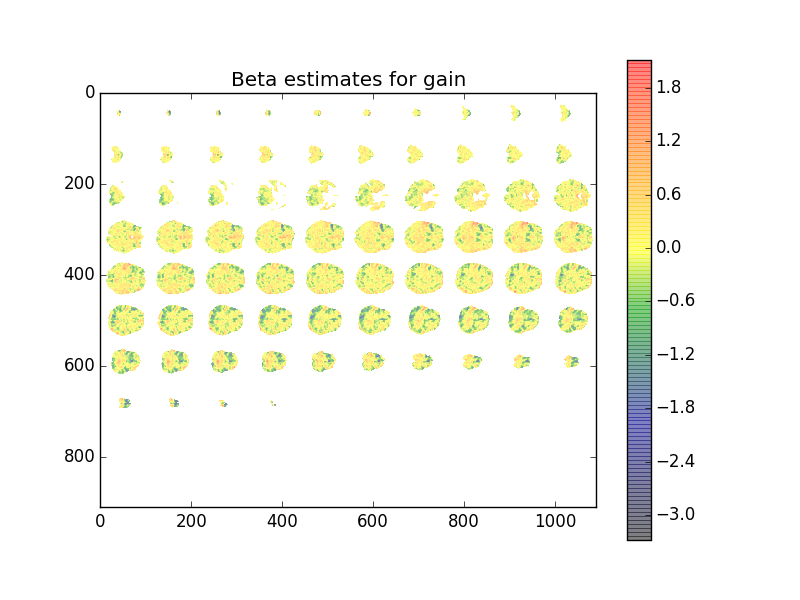
\includegraphics[width=100mm]{images/parameter_map_gain.png}               
\caption{Parameter Map Corresponding to Parametric Gain}
\label{fig:beta1}
\end{figure}

\begin{figure}[h!]
\centering
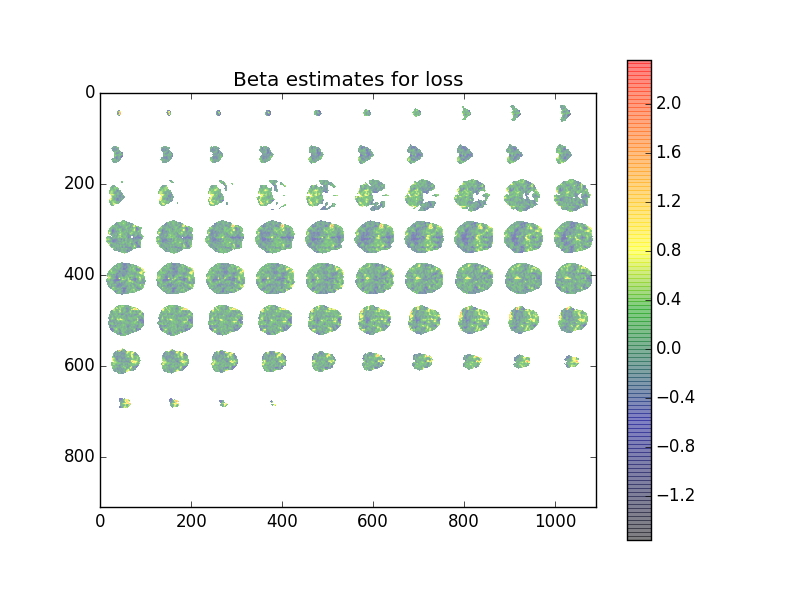
\includegraphics[width=100mm]{images/parameter_map_loss.png}               
\caption{Parameter Map Corresponding to Parametric Loss}
\label{fig:beta2}
\end{figure}

\begin{figure}[h!]
\centering
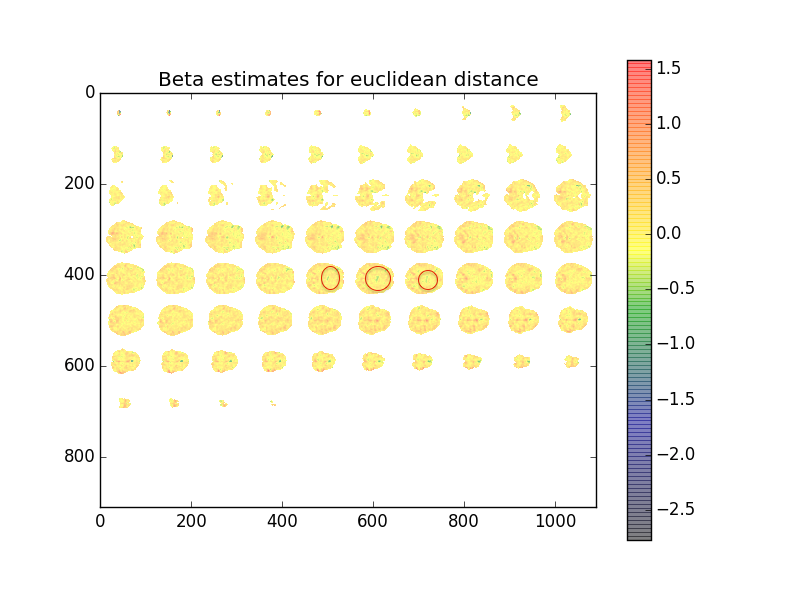
\includegraphics[width=100mm]{images/parameter_map_dist.png}               
\caption{Parameter Map Corresponding to Distance from Indifference}
\label{fig:beta3}
\end{figure}

\begin{figure}[h!]
\centering
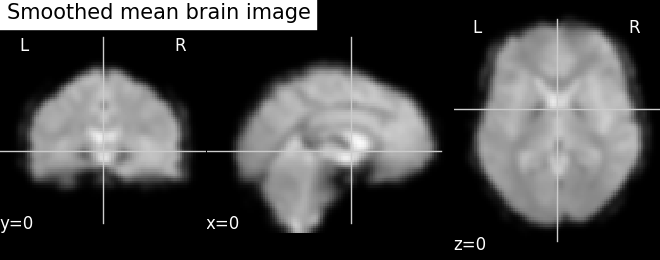
\includegraphics[width=120mm]{images/brain_template.png}               
\caption{Background Image for t-statistic and p-value map}
\label{fig:brain_temp}
\end{figure}

\begin{figure}[h!]
\centering
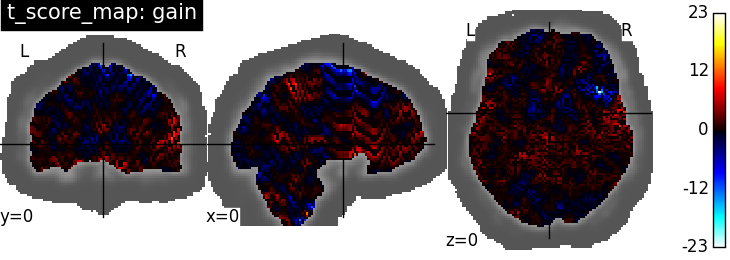
\includegraphics[width=100mm]{images/t_scores_gain.png}               
\caption{t-score map (gain)}
\label{fig:t_gain}
\end{figure}

\begin{figure}[h!]
\centering
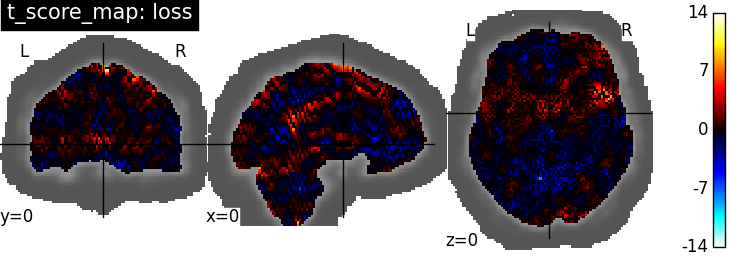
\includegraphics[width=100mm]{images/t_scores_loss.png}               
\caption{t-statistic map (loss)}
\label{fig:t_loss}
\end{figure}

\begin{figure}[h!]
\centering
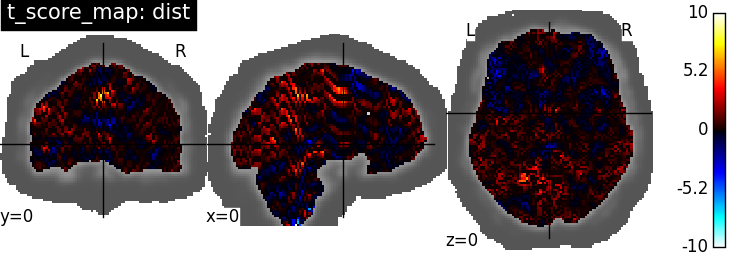
\includegraphics[width=100mm]{images/t_scores_dist.png}               
\caption{t-statistic map (dist)}
\label{fig:t_dist}
\end{figure}

\begin{figure}[h!]
\centering
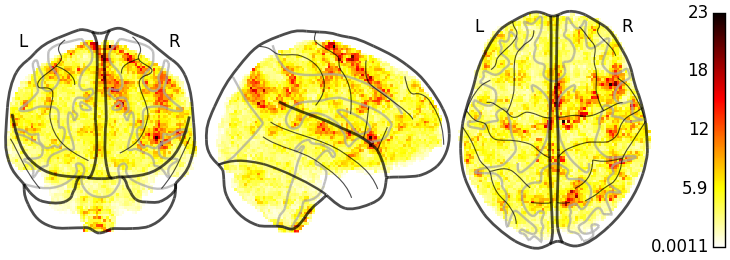
\includegraphics[width=100mm]{images/t_glass_brain_gain.png}               
\caption{t value corresponding to gain on glass brain}
\label{fig:t_glass1}
\end{figure}

\begin{figure}[h!]
\centering
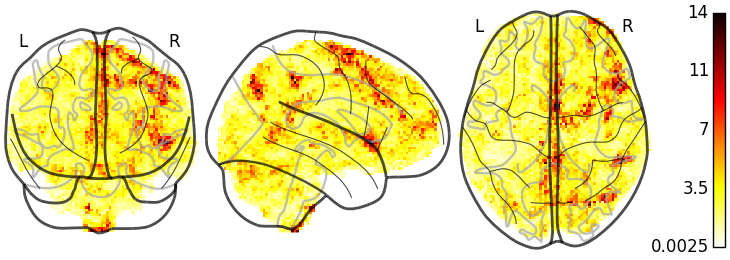
\includegraphics[width=100mm]{images/t_glass_brain_loss.png}               
\caption{t value corresponding to loss on glass brain}
\label{fig:t_glass2}
\end{figure}

\begin{figure}[h!]
\centering
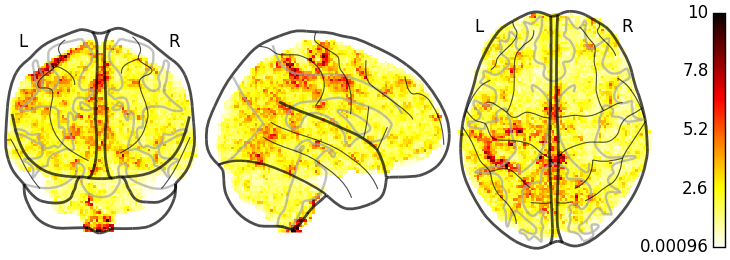
\includegraphics[width=100mm]{images/t_glass_brain_dist.png}               
\caption{t value corresponding to distance on glass brain}
\label{fig:t_glass3}
\end{figure}